% !TEX TS-program = pdflatexmk
% !BIB program = bibtex 
%% -- Chapter A-I (anpassen an die Realität)
%% --
\documentclass[%
,12pt		% für Korrekturen % wegmachen und Zeilenabstand größer machen
,oneside]{book}

%% --
%\usepackage{setspace}
%\doublespacing 

%% -- Gemeinsame Pakete und Definitionen
%% --
%% -- Stand 2025/02/05
%% --
%% Welche Pakete verwenden wir 
%% -- 
\usepackage{graphicx}        
\usepackage{libertine}

%% -- Nummerierung Abschnittsweise
%% --
\renewcommand\thesection{\arabic{section}}
\renewcommand\thesubsection{\thesection.\arabic{subsection}}

%% -- AMS-math und mathtools
%% --
\usepackage{amsmath, amssymb, amsthm}	
\usepackage{mathtools}

%% -- Die Theorem-Umgebungen: Nummerierung nach Abschnitten
%% --

%% --
\theoremstyle{plain}
\newtheorem{theorem}{Theorem}[section]
\newtheorem{proposition}[theorem]{Proposition}
\newtheorem{corollary}[theorem]{Corollary}
\newtheorem{lemma}[theorem]{Lemma} 
%% --
\theoremstyle{definition}
\newtheorem{example}[theorem]{Example}
\newtheorem{examples}[theorem]{Examples} 
\newtheorem{definition}[theorem]{Definition}
%% --
\theoremstyle{remark}
\newtheorem{remark}[theorem]{Remark}
\newtheorem{remarks}[theorem]{Remarks}



%% -- Unsere Pakete
%% --
\usepackage[english]{babel}					% Trennungen richtig
\usepackage{csquotes}						% \enquote{Text} 
\usepackage[inline,shortlabels]{enumitem}	% \begin{enumerate}[(i)] oder [(a)] 
	\setlist{parsep=0.0em}					% etwas enger		
\usepackage{ragged2e}						% \RaggedRight = Flattersatz
%% --
\usepackage{tikz}
\usepackage{tikz-cd}
\usetikzlibrary{matrix,arrows.meta,calc}
%% --
\usepackage{comment}
\usepackage{xspace}

%% --

\usepackage{hyperref}
\hypersetup{
    colorlinks=true,
    linkcolor=blue,
    citecolor=blue,
    urlcolor=blue,
    linktoc=all
}


  


%% -- Gemeinsame Abkürzungen
%% --
%% -- Definitionen
%% --
%% -- Zahlen
\newcommand{\N}{\mathbb{N}}		% Natuerliche Zahlen
\newcommand{\Z}{\mathbb{Z}}		% Ganze Zahlen
\newcommand{\Q}{\mathbb{Q}}		% Rationale Zahlen
\newcommand{\R}{\mathbb{R}}		% Reelle Zahlen
\newcommand{\C}{\mathbb{C}}		% Komplexe Zahlen
\newcommand{\K}{\mathbb{K}}		% Koerperzeichen
\newcommand{\T}{\mathbb{T}}

%% -- Operatoren					
\DeclareMathOperator{\Id}{Id}
\DeclareMathOperator{\sign}{sign}


%% -- Differential Allgemeine Abkuerzungen
%% --
\newcommand*{\diff}[1]{\mathop{}\!\mathrm{d}{#1}}	% \diff{s} = ds, 
\renewcommand*{\d}[1]{\mathop{}\!\mathrm{d}{#1}}	% \d{\mu} = d.., 
\newcommand*{\ds}{\mathop{}\!\mathrm{d}{s}}       	% \ds = ds, 
\newcommand*{\dg}{\mathop{}\!\mathrm{d}{g}}       	% \dg = dg, 
\newcommand*{\dt}{\mathop{}\!\mathrm{d}{t}}       	% \dt = dt, 
\newcommand*{\dx}{\mathop{}\!\mathrm{d}{x}}       	% \dx = dx, 
\newcommand*{\dy}{\mathop{}\!\mathrm{d}{y}}       	% \dy = dy, 
\newcommand*{\dr}{\mathop{}\!\mathrm{d}{r}}       	% \dx = dr, 

%% --
\newcommand{\LE}{\mathcal{L}(E)} 		% 
\renewcommand{\L}[1]{\mathcal{L}(#1)} 	% \L{C(K)} zum Beispiel


%% -- Enpunkt korrekt
\newcommand*{\eg}{e.g.\xspace}
\newcommand*{\ie}{i.e.\xspace}
\newcommand*{\resp}{resp.\xspace}
\newcommand*{\vs}{vs.\xspace}
\newcommand*{\cf}{cf.\xspace}

%% --
\newcommand{\CA}{$\mathrm{C}^{*}$}
\newcommand{\WA}{$\mathrm{W}^{*}$}

%% --
\newcommand{\rank}{\mathop{}\!\mathrm{Rang}\,}

%%
\newcommand*{\TT}{\mathcal{T}}
\newcommand*{\F}{\mathcal{F}}



%% -- Index für später
%% --

\usepackage{imakeidx}
\makeindex[columns=2, options=-s svind.ist]


%% -- Literatur
%% -- für später

%\usepackage[round]{natbib}
%%\bibliographystyle{spmpsci}
%\bibliographystyle{abbrvnat}

%% --

\usepackage{hyperref}
\hypersetup{%
,colorlinks=true 
,linkcolor=blue
,citecolor=blue
,urlcolor=blue
,linktoc=all
%,hidelinks=true
}


          
%% --
           
\begin{document}
%\tableofcontents

\setcounter{chapter}{0}		%% anpassen 1/2/3 -> Chapter 2/3/4
\setcounter{section}{1}		%% immer

% !TEX TS-program = pdflatexmk
% !TEX root = chap-a1-test.tex
% !BIB program = bibtex
%% --
%% -- Chapter A-I
%% -- Stand: 2025/02/20
%% --
%\setcounter{chapter}{0}

\chapter[Basic Results on Semigroups on Banach Spaces]{Basic Results on Semigroups on Banach Spaces}\label{chap:a1}
%\normalsize{\hspace{2cm} R. Nagel \& U. Schlotterbeck}}
\index{Basic Results}
%% --
Since the basic theory of one-parameter semigroups can be found in several excellent books (e.g. \citet{davies:1980}, \citet{goldstein:1985a}, \citet{pazy:1983} or \citet{hillephillips:1957}), we do not want to give a self-contained introduction to this subject here.
It may however be useful to fix our notation, to collect briefly some important definitions and results (Section 1), to present a list of \emph{standard examples} in Section~\ref{sec:a1-2} %(Section 2) 
and to discuss standard constructions of new semigroups from a given one in Section~\ref{sec:a1-3} on p.\,\pageref{sec:a1-3}. %(Section 3).

In the entire chapter we denote by $E$ a (real or) complex Banach space and consider one-parameter semigroups of bounded linear operators $T(t)$ on $E$.
By this we understand a subset $\{T(t) \colon  t \in \R_{+}\}$ of $\LE$, usually written as $(T(t))_{t\geq0}$, such that
%% --
\begin{align*}
	T(0) &= \Id, \\
	T(s+t) &= T(s) \cdot T(t) \text{ for all $s$, $t \in \R_{+}$.}
\end{align*}
%% --
In more abstract terms this means that the map $t \mapsto T(t)$ is a homomorphism from the additive semigroup $(\R_{+},+)$ into the multiplicative semigroup $(\LE,\cdot)$.
Similarly, a one-parameter group $(T(t))_{t\in\R}$ will be a homomorphic image of the group $(\R,+)$ in $(\LE,\cdot)$.
%% --
\section{Standard Definitions and Results}\label{sec:a1-1}
\index{Basic Results!Standard Definitions and Results}
%% --
We consider a one-parameter semigroup $(T(t))_{t \geq 0}$ on a Banach space $E$ 
and observe that the domain $\R_{+}$ and the range $\LE$ of the (semigroup) homomorphism $\tau \colon t \mapsto T(t)$ are topological semigroups for the natural topology on $\R_{+}$ and any one of the standard operator topologies on $\LE$.
We single out the strong operator topology on $\LE$ and require $\tau$ to be continuous.
%% --
\begin{definition}\label{def:a1-1.1}
A one-parameter semigroup $(T(t))_{t\geq0}$ is called \emph{strongly continuous} if the map $t \mapsto T(t)$ is continuous for the strong operator topology on $\LE$, \eg
%% --
\[
	\lim_{t\to t_{0}} \|T(t)f - T(t_{0})f\| = 0
\]
%% --
for every $f \in E$ and $t$, $t_{0} \geq 0$.
\end{definition}
%% --
Clearly one defines in a similar way \emph{weakly continuous}, \resp \emph{uniformly continuous} (compare A-II, Def. 1.19) semigroups, but since we concentrate on the strongly continuous case we agree on the following terminology.
%% --
\begin{quote}
If not stated otherwise, a \emph{semigroup} is a strongly continuous one-parameter semigroup of bounded linear operators.
\end{quote}
%% --
Next we collect a few elementary facts on the continuity and boundedness of one-parameter semigroups.
%% --
\begin{remarks}\label{rem:a1-1.2}
%% --
\begin{enumerate}[(i), wide, labelsep=1em, itemindent=\parindent]

\item 
A one-parameter semigroup $(T(t))_{t \geq 0}$ on a Banach space $E$ is strongly continuous if and only if for any $f \in E$ it is true that $T(t)f \to f$ if $t \to 0$.

\item 
For every strongly continuous semigroup there exist constants $M \geq 1$, $w \in \R$ such that $\|T(t)\| \leq M \cdot e^{wt}$ for every $t \geq 0$.
\item If $(T(t))_{t\geq0}$ is a one-parameter semigroup such that $\|T(t)\|$ is bounded for $0 < t \leq \delta$ then it is strongly continuous if and only if $\lim_{t \to 0} T(t)f = f$ for every $f$ in a total subset of $E$.
\end{enumerate}
\end{remarks}
%% --
The exponential estimate from Remark~\ref{rem:a1-1.2}\,(ii) for the growth of $\|T(t)\|$ can be used to define an important characteristic of the semigroup.
%% --
\begin{definition}\label{def:a1-1.3}
By the growth bound (or type) of the semigroup $(T(t))_{t\geq0}$ we understand the number
%% --
\begin{align*}\label{eq:a1-1.1}
\omega_{0} \coloneqq{}& \inf\{w \in \R \colon \text{There exists } M \in \R_{+} \text{ such that } \|T(t)\| \leq Me^{wt} \text{ for } t \geq 0\} \\
={}& \lim_{t\to\infty} \frac{1}{t}\log\|T(t)\| = \inf_{t>0} \frac{1}{t}\log\|T(t)\| \notag .
\end{align*}
%% --
\end{definition}
%% --
\noindent Particularily important are semigroups such that for every $t \geq 0$ we have $\|T(t)\| \leq M$ (\emph{bounded semigroups}) or $\|T(t)\| \leq 1$ (\emph{contraction semigroups}).
In both cases we have $\omega_{0} \leq 0$.

It follows from the subsequent examples and from Def.~\ref{def:a1-1.3} that $\omega_{0}$ may be any number $ -\infty \leq \omega < +\infty$.
Moreover the reader should observe that the infimum in Def.~\ref{def:a1-1.3} need not be attained and that $M$ may be larger than $1$ even for bounded semigroups.
%% --
\begin{examples}\label{ex:a1-1.4}
%% --
\begin{enumerate}[(i), wide, labelsep=1em, itemindent=\parindent]

\item 
Take $E = \mathbb{C}^2$, 
\[
	A = \begin{pmatrix}0 & 1\\0 & 0\end{pmatrix} 
	\quad \text{and} \quad 
	T(t) = e^{tA} = \begin{pmatrix}1 & t\\0 & 1\end{pmatrix} .
\]
%
Then for the $\ell^{1}$-norm on $E$ we obtain $\|T(t)\| = 1 + t$, hence $(T(t))_{t\geq0}$ is an unbounded semigroup having growth bound $\omega_{0} = 0$.

\item 
Take $E = L^1(\R)$ and for $f \in E$, $t \geq 0$ define
%% --
\begin{align*}
T(t)f(x) \coloneqq 
	\begin{cases}
		2\cdot f(x+t) & \text{if } x \in [-t,0] \\
		f(x+t) & \text{otherwise}.
	\end{cases}
\end{align*}
%% --
Each $T(t)$, $t > 0$, satisfies $\|T(t)\| = 2$ as can be seen by taking $f := \chi_{[0,t]}$.
Therefore $(T(t))_{t \geq 0}$ is a strongly continuous semigroup which is bounded, hence has $\omega_{0} = 0$, but the constant $M$ in (1.3) cannot be chosen to be $1$.

\end{enumerate}
\end{examples}
%% --
The most important object associated to a strongly continuous semigroup $(T(t))_{t\geq0}$ is its \emph{generator} which is obtained as the (right)derivative of the map $t \mapsto T(t)$ at $t = 0$.
Since for strongly continuous semigroups the functions $t \mapsto T(t)f$, $f \in E$, are continuous but not always differentiable, we have to restrict our attention to those $f \in E$ for which the desired derivative exists.
We then obtain the \emph{generator} as a not necessarily everywhere defined operator.

\begin{definition}\label{def:a1-1.5}
To every semigroup $(T(t))_{t \geq 0}$ there belongs an operator $(A,D(A))$, called the \emph{generator} and defined on the \emph{domain}
%% --
\begin{align*}
	D(A) \coloneqq{} & \{f \in E \colon \lim_{h\to0} \frac{T(h)f - f}{h} \text{ exists in $E$}\} \text{ by} \\
	Af \coloneqq{} & \lim_{h\to0} \frac{T(h)f - f}{h} \quad (f \in D(A)).
\end{align*}
%% --
\end{definition}
%% --
\noindent Clearly, $D(A)$ is a linear subspace of $E$ and $A$ is linear from $D(A)$ into $E$.
Only in certain special cases (see \ref{subsec:a1-2.1}) the generator
is everywhere defined and therefore bounded (use Prop.~\ref{prop:a1-1.9}\,(ii)) on p.\,\pageref{prop:a1-1.9}). %Prop.1.9(i)).
In general, the precise extent of the domain $D(A)$ is essential for the characterization of the generator.
But since the domain is canonically associated to the generator of a semigroup, we shall write in most cases $A$ instead of $(A,D(A))$.

As a first result we collect some information on the domain of the generator.
%% --
\begin{proposition}\label{prop:a1-1.6}
For the generator $A$ of a semigroup $(T(t))_{t \geq 0}$ on a Banach space~$E$ the following assertions hold.
%% --
\begin{enumerate}[(i)]
\item
If $f \in D(A)$, then $T(t)f \in D(A)$ for every $t \geq 0$.

\item
The map $t \mapsto T(t)f$ is differentiable on $\R_{+}$ if and only if $f \in D(A)$.
In that case one has
%% --
\begin{equation}\label{eq:a1-1.2}
    \frac{d}{dt} T(t)f = AT(t)f = T(t)Af .
\end{equation}
%% --
\item
For every $f \in E$ and $t > 0$ the element $\int_0^t T(s)f\ds$ belongs to $D(A)$ and one has
%% --
\begin{equation}\label{eq:a1-1.3}
    A\int_0^t T(s)f \ds = T(t)f - f  .
\end{equation}
%% --
\item
If $f \in D(A)$, then
%% --
\begin{equation}\label{eq:a1-1.4}
    \int_0^t T(s)Af \ds = T(t)f - f  .
\end{equation}

%% --
\item
The domain $D(A)$ is dense in $E$.
\end{enumerate}
%% --
\end{proposition}
%% --
The identity \eqref{eq:a1-1.2} is of great importance and shows how semigroups are related to certain Cauchy problems.
We state this explicitly in the following theorem.
%% --
\begin{theorem}\label{thm:a1-1.7}
Let $(A,D(A))$ be the generator of a strongly continuous semigroup $(T(t))_{t \geq 0}$ on the Banach space $E$.
Then the \emph{abstract Cauchy problem}
%% --
\begin{equation}\label{eq:a1-1.5}
\frac{d}{dt}\xi(t) = A\xi(t), \quad \xi(0) = f_{0}
\end{equation}
%% --
has a unique solution $\xi \colon \R_{+} \to D(A)$ in $C^1(\R_{+},E)$ for every $f_{0} \in D(A)$.
In fact, this solution is given by $\xi(t) \coloneqq T(t)f_{0}$.
\end{theorem}
%% --
For more on the relation of semigroups to abstract Cauchy problems we refer to A-II,Section 1.
Here we only point out that the above theorem implies that a semigroup is uniquely determined by its generator.

While the generator is bounded only for uniformly continuous semigroups (see Sec.\,\ref{sec:a1-2} below), it always enjoys a weaker but useful property.
%% --
\begin{definition}\label{def:a1-1.8}
An operator $B$ with domain $D(B)$ on a Banach space $E$ is called \emph{closed} if $D(B)$ endowed with the \emph{graph norm}
%% --
\[
    \|f\|_{B} \coloneqq \|f\| + \|Bf\|
\]
%% --
becomes a Banach space.
Equivalently, $(B,D(B))$ is closed if and only if its \emph{graph} $\{(f,Bf) \colon f \in D(B)\}$ is closed in $E \times E$, i.e.\xspace,
%% --
\[
    f_{n} \in D(B), f_{n} \to f \text{ and } Bf_{n} \to g \text{ implies } f \in D(B) \text{ and } Bf = g.
\]
%% --
\end{definition}
%% --
It is clear from this definition that the \emph{closedness} of an operator $B$ depends very much on the size of the domain $D(B)$.
For example, a bounded and densely defined operator $(B,D(B))$ is closed if and only if $D(B) = E$.

On the other hand it may happen that $(B,D(B))$ is not closed but has a closed \emph{extension} $(C,D(C))$, i.e.\xspace  $ D(B) \subseteq D(C)$ and $Bf = Cf$ for every $f \in D(B)$.
In that case, $B$ is called \emph{closable}, a property which is equivalent to
%% --
\[
    f_{n} \in D(B), f_{n} \to 0 \text{ and } Bf_{n} \to g \text{ implies } g = 0.
\]
%% --
The smallest closed extension of $(B,D(B))$ will be called the \emph{closure} $\overline{B}$ with domain $D(\overline{B})$.
In other words, the graph of $\overline{B}$ is the closure of $\{(f,Bf) \colon f \in D(B)\}$ in $E \times E$.

Finally we call a subset $D_{0}$ of $D(B)$ a \emph{core} for $B$ if $D_{0}$ is $\|\cdot\|_{B}$-dense in $D(B)$.
This means that a closed operator is determined (via closure) by its restriction to a core in its domain.

We now collect the fundamental topological properties of semigroup generators, their domains (see also A-II,Cor.1.34) and their resolvents.
%% --
\begin{proposition}\label{prop:a1-1.9}
For the generator $A$ of a strongly continuous semigroup $(T(t))_{t \geq 0}$ the following hold.
%% --
\begin{enumerate}[(i)]
\item 
The generator $A$ is a closed operator.

\item
If a subspace $D_{0}$ of the domain $D(A)$ is dense in $E$ and $(T(t))$-invariant, then it is a core for $A$.
% --
\item Define $D(A^{n}) \coloneqq \{f \in D(A^{n-1}) \colon Af \in D(A^{n-1})\}$, $D(A^{1}) = D(A)$.
Then $D(A^{\infty}) \coloneqq \bigcap_{n \in \N} D(A^{n})$ is dense in $E$ and a core for $A$.
\end{enumerate}
%% --
\end{proposition}
%% --
\begin{example}\label{ex:a1-1.10}
Property (iii) above does not hold for general densely defined closed operators.
Take $E = C\left[ 0,1 \right]$, $D(B) = C^{1}\left[ 0,1 \right]$ and $Bf = q \cdot f'$ for some nowhere differentiable function $q \in C\left[ 0,1 \right]$.
Then $B$ is closed, but $D(B^{2}) = \{0\}$.
\end{example}
%% --

%% --
\begin{proposition}\label{prop:a1-1.11}
For the generator $A$ of a strongly continous semigroup on a Banach space $E$ the following hold.

If $\int_{0}^{\infty} e^{-\lambda t}T(t)f \, dt$ exists for every $f \in E$ and some $\lambda \in \mathbb{C}$, then $\lambda \in \rho(A)$ and $R(\lambda,A)f = \int_{0}^{\infty} e^{-\lambda t}T(t)f \, dt$.
In particular,
%% --
\begin{equation}\label{eq:a1-1.7}
R(\lambda,A)^{n+1}f = \frac{(-1)^{n}}{n!}\left(\frac{d}{d\lambda}\right)^{n} R(\lambda,A)f = \int_{0}^{\infty} e^{-\lambda t}\frac{t^{n}}{n!}T(t)f \, dt
\end{equation}
%% --
for every $f \in E$, $n \geq 0$ and $\lambda \in \mathbb{C}$ with $\Re(\lambda) > \omega$.
\end{proposition}
%% --
%% --
\begin{remarks}\label{rem:a1-1.12}

\begin{enumerate}[(i), wide, labelsep=1em, itemindent=\parindent]

\item 
For continuous Banach space valued functions such as $t \mapsto T(t)f$ we consider the Riemann integral and define 
%% --
\[
\int_{0}^{\infty}T(t)f \, \dt 
\quad \text{as} \quad
\lim_{t \to \infty}\int_{0}^{t}T(s)f \, \ds .
\]
%% --
Sometimes such integrals for strongly continuous semigroups are written as $\int_{a}^{b}T(t) \, dt$ but understood in the strong sense.

\item 
Since the generator $(A,D(A))$ determines the semigroup uniquely, we will speak occasionally of the growth bound of the generator instead of the semigroup, i.e.\xspace we write $\omega_{0} = \omega_{0}(A) = \omega_{0}((T(t))_{t \geq 0}$.

\item 
For one-parameter groups it might seem to be more natural to define the generator as the \emph{derivative} rather than just the \emph{right derivative} at $t = 0$.
This yields the same operator as the following result shows.

The strongly continuous semigroup $(T(t))_{t \geq 0}$ with generator $A$ can be extended to a strongly continuous one-parameter group $(U(t))_{t \in \R}$ if and only if $-A$ generates a semigroup $(S(t))_{t \geq 0}$.

In that case $(U(t))_{t \in \R}$ is obtained as
%% --
\[
    U(t) = \begin{cases}
        T(t) & \text{for } t \geq 0 ,\\
        S(-t) & \text{for } t \leq 0 .
    \end{cases}
\]
%% --
We refer to \citet[Prop.1.14]{davies:1980} for the details.

\end{enumerate}
\end{remarks}
%% --
\section{Standard Examples}\label{sec:a1-2}
\index{Basic Results!Standard Examples}
%\index{Standard Examples}
%% --
In this section we list and discuss briefly the most basic examples of semigroups together with their generators.
These semigroups will reappear throughout this book and will be used to illustrate the theory.
We start with the class of semigroups mentioned after Definition~\ref{def:a1-1.1} on p.~\pageref{def:a1-1.1}.
%% --
\subsection{Uniformly Continuous Semigroups}\label{subsec:a1-2.1}
%\index{Uniformly Continuous Semigroups}
%\index{Semigroups!Uniformly Continuous}
\index{Standard Examples!Uniformly Continuous Semigroups}
%% --
It follows from elementary operator theory that for every bounded operator $A$ in  $\LE$ the sum
%% --
\[
    \sum_{n=0}^{\infty} \frac{t^{n}A^{n}}{n!} = \colon e^{tA}
\]
%% --
exists and determines a unique uniformly continuous (semi)group $(e^{tA})_{t \in \R}$ having $A$ as its generator.
Conversely, any uniformly continuous semigroup is of this form.

If the semigroup $(T(t))_{t \geq 0}$ is uniformly continuous, then $\frac{1}{t}\int_{0}^{t} T(s) \ds$ uniformly converges to $T(0) = \Id$ as $t \to 0$.
Therefore for some $t' > 0$ the operator $\frac{1}{t'}\int_{0}^{t'} T(s) \ds$ is invertible and every $f \in E$ is of the form $f = \frac{1}{t'}\int_{0}^{t'} T(s)g \ds$ for some $g \in E$.
But these elements belong to $D(A)$ by (1.3), hence $D(A) = E$.
Since the generator $A$ is closed and everywhere defined, it must be bounded.

Remark that bounded operators are always generators of groups, not just semigroups.
Moreover, the growth bound $\omega$ satisfies $|\omega| \leq \|A\|$ in this situation.

The above characterization of the generators of uniformly continuous semigroups as the bounded operators shows that these semigroups are---at least in many aspects---rather simple objects.
%% --
\subsection{Matrix Semigroups}\label{subsec:a1-2.2}
%\index{Matrix Semigroups}
%\index{Semigroups!Matrix}
\index{Standard Examples!Matrix Semigroups}
%% --
The above considerations expecially apply in the situation $E = \mathbb{C}^{n}$.
If $n = 2$ and $A = (a_{ij})_{2 \times 2}$ the following explicit formulas for $e^{tA}$ might be of interest.

Set
%% --
\begin{enumerate*}[(i)]
\item
$s \coloneqq \text{trace } A$, 

\item
$d \coloneqq \text{det } A$

\item
and $D \coloneqq (s^{2} - 4d)^{1/2}$.
\end{enumerate*}
%% --
Then if  $D \neq 0$
%% -- 
\[
    e^{tA} = 
        e^{ts/2} \cdot [D^{-1}2\sinh(tD/2) \cdot A + (\cosh(tD/2) - sD^{-1}\sinh(tD/2)) \cdot \Id] 
\]
%% --
and if $D=0$
%% --
\[
	e^{ts/2} \cdot [tA + (1 - ts/2) \cdot \Id] .
\]
%% --

%% --
\subsection{Multiplication Semigroups}\label{subsec:a1-2.3}
%\index{Multiplication Semigroups}
%\index{Examples!Multiplication Semigroups}
\index{Standard Examples!Multiplication Semigroups}
%% --
Many Banach spaces appearing in applications are Banach spaces of (real or) complex valued functions over a set $X$.
%% --
As the most standard examples of these \enquote{function spaces}, we mention the space $C_{0}(X)$ of all continuous complex valued functions vanishing at infinity on a locally compact space $X$, or the spaces $L^{p}(X,\Sigma,\mu)$, $1 \leq p \leq \infty$, of all (equivalence classes of) $p$-integrable functions on a $\sigma$-finite measure space $(X,\Sigma,\mu)$.

On these function spaces $E = C_{0}(X)$, \resp $E = L^{p}(X,\Sigma,\mu)$, there is a simple way to define \emph{multiplication operators}.

Take a continuous, \resp measurable function $q \colon X \to \mathbb{C}$ and define
%% --
\[
    M_{q}f \coloneqq q \cdot f, \quad \text{i.e.\xspace} \quad M_{q}f(x) 
    \coloneqq q(x) 	\cdot f(x) \quad \text{for } x \in X 
\]
%% --
and for every $f$ in the \emph{maximal} domain $D(M_{q}) \coloneqq \{g \in E \colon q \cdot g \in E\}$.

This natural domain is a dense subspace of $C_{0}(X)$, \resp $L^{p}(X,\Sigma,\mu)$, for $1 \leq p < \infty$.
Moreover, $(M_{q},D(M_{q}))$ is a closed operator.
This is easy in case $E = C_{0}(X)$.

For $E = L^{p}(X,\Sigma,\mu)$, $1 \leq p < \infty$, we consider a sequence $(f_{n}) \subset E$ such that $\lim_{n \to \infty} f_{n} = f \in E$ and $\lim_{n \to \infty} qf_{n} = \colon g \in E$.
Choose a subsequence $(f_{n(k)})_{k \in \N}$ such that $\lim_{k \to \infty} f_{n(k)}(x) = f(x)$ and $\lim_{k \to \infty} q(x)f_{n(k)}(x) = g(x)$ for $\mu$-almost every $x \in X$.
Then $g = q \cdot f$ and $f \in D(M_{q})$, i.e.\xspace $M_{q}$ is closed.

For such multiplication operators many properties can be checked quite directly.
For example, the following statements are equivalent.
%% --
\begin{enumerate}[(a)]
\item 
$M_{q}$ is bounded.

\item 
$q$ is ($\mu$-essentially) bounded.
\end{enumerate}
%% --
One has $\|M_{q}\| = \|q\|_{\infty}$ in this situation.

Observe that on spaces $C(K)$, $K$ compact, there are no densely defined, unbounded multiplication operators.

By defining the multiplication semigroups
%% --
\[
    T(t)f(x) \coloneqq \exp(t \cdot q(x))f(x), \quad x \in X, f \in E,
\]
%% --
one obtains the following characterizations.

%% --
\begin{proposition}\label{prop:a1-2.3}
%\index{Multiplication Operators}
%\index{Operators!Multiplication}
\index{Standard Examples!Multiplication Operators}
%% --
Let $M_{q}$ be a multiplication operator on $E = C_{0}(X)$ or $E = L^{p}(X,\Sigma,\mu)$, $1 \leq p < \infty$.
Then the properties (a) and (b), \resp (a') and (b'), are equivalent.
%% --
\begin{enumerate}[(a)]
\item 
	$M_{q}$ generates a strongly continuous semigroup.

\item 
	$\sup\{\Re( q(x)) \colon x \in X \} < \infty$.

\item[(a')] 
	$M_{q}$ generates a uniformly continuous semigroup.

\item[(b')] 
	$\sup\{|q(x)| \colon x \in X \} < \infty$.
\end{enumerate}
%% --
\end{proposition}
%% --
As a consequence one computes the growth bound of a multiplication semigroup as
%% --
\[
    \omega_{0} = \sup\{\Re(q(x)) \colon x \in X\} 
\]
%% --
in the case $E = C_{0}(X)$ and 
%% --
\[
    \omega_{0} = \mu\text{-ess-}\sup\{\Re(q(x)) \colon x \in X\} 
\]
%% --
in the case  $E = L^{p}(\mu)$.
It is a nice exercise to characterize those multiplication operators which generate strongly continuous groups.

We point out that the above results cover the cases of sequence spaces such as $c_{0}$ or $\ell^{p}$, $1 \leq p < \infty$.
An abstract characterization of generators of multiplication semigroups will be given in C-II,Thm.5.13.

%% --
\subsection{Translation (Semi)Groups}\label{subsec:a1-2.4}
%\index{Translation Semigroups}
%\index{Semigroups!Translation}
\index{Standard Examples!Translation Semigroups}
%% --

Let $E$ to be one of the following function spaces $C_{0}(\R_{+})$, $C_{0}(\R)$ or $L^{p}(\R_{+})$, $L^{p}(\R)$ for $1 \leq p < \infty$.
Define $T(t)$ to be the (left) translation operator
%% --
\[
    T(t)f(x) \coloneqq f(x+t)
\]
%% --
for $x$ ,, $ t \in \R_{+}$, \resp $x, t \in \R$ and $f \in E$.
Then $(T(t))_{t \geq 0}$ is a strongly continous semigroup, \resp group of contractions on $E$ and its generator is the first derivative $\frac{d}{dx}$ with \emph{maximal} domain.
In order to be more precise we have to distinguish the cases $E = C_{0}$ and $E = L^{p}$.
%% -- 

The generator of the translation (semi)group on $E = C_{0}(\R_{+})$ is 
%% --
\begin{align*}
    Af & \coloneqq \frac{d}{\dx}f = f' \\
    D(A) &\coloneqq \{f \in E \colon f \text{ differentiable and } f' \in E\}.
\end{align*}
%% --
\begin{proof}
For $f \in D(A)$ it follows that for every $x \in \R_{(+)}$
%% --
\[
    \lim_{h \to 0} \frac{T(h)f(x) - f(x)}{h} = \lim_{h \to 0} \frac{f(x+h) - f(x)}{h} \text{ exists}
\]
%% --
(uniformly in $x$) and coincides with $Af(x)$.
Therefore $f$ is differentiable and $f' \in E$.

On the other hand, take $f \in E$ differentiable such that $f' \in E$.
Then
%% --
\[
    \left|\frac{f(x+h) - f(x)}{h} - f'(x)\right| \leq \frac{1}{h}\int_{x}^{x+h}|f'(y) - f'(x)|\,\dy,
\]
%% --
where the last expression tends to zero uniformly in $x$ as $h \to 0$.
Thus $f \in D(A)$ and $f' = Af$.
\end{proof}
%% --
The generator of the translation (semi)group on $E = L^{p}(\R_{+})$, $1 \leq p < \infty$, is
%% --
\begin{align*}
    Af &\coloneqq \frac{d}{\dx}f = f', \\
    D(A) &\coloneqq \{f \in E \colon f \text{ absolutely continuous}, f' \in E\}.
\end{align*}
%% --
\begin{proof}
Take $f \in D(A)$ such that $\lim_{h \to 0} \frac{1}{h}(T(h)f - f) = g \in E$.
Since integration is continuous, we obtain for every $a$, $b \in \R_{(+)}$ that
%% --
\begin{equation*}\label{eq:a1-2.1}
(*) \quad \frac{1}{h}\int_{b+h}^{b} f(x) \dx - \frac{1}{h}\int_{a+h}^{a} f(x) \dx = \int_{a}^{b} \frac{f(x+h) - f(x)}{h} \dx
\end{equation*}
%% --
converges to $\int_{a}^{b} g(x) \dx$ as $h \to 0+$.
But for almost all $a, b$ the left hand side of $(*)$ converges to $f(b) - f(a)$.
By redefining $f$ on a nullset we obtain
%% --
\[
    f(y) = \int_{a}^{y} g(x)\dx + f(a), \quad y \in \R_{(+)},
\]
%% --
which is an absolutely continuous function whose derivative is (almost everywhere) equal to $g$.

On the other hand, let $f$ be absolutely continuous such that $f' \in L^{p}$.
Then
%% --
\begin{align*}
    \lim_{h \to 0} \int \left|\frac{f(x+h) - f(x)}{h} - f'(x)\right|^{p} \dx 
    &= \lim_{h \to 0} \int \left|\frac{1}{h}\int_{0}^{h} (f'(x+s) - f'(x)) \ds\right|^{p} \dx \\
    &= \lim_{h \to 0} \int \left|\int_{0}^{1} (f'(x+uh) - f'(x)) \du\right|^{p} \dx \\
    &\leq \lim_{h \to 0} \int \int_{0}^{1} |f'(x+uh) - f'(x)|^{p} \du \dx \\
    &= \int_{0}^{1} \lim_{h \to 0} \int |f'(x+uh) - f'(x)|^{p} \dx \du = 0,
\end{align*}
%% --
hence $f \in D(A)$.
\end{proof}
%% --
\subsection{Rotation Groups}\label{subsec:a1-2.5}
%\index{Rotation Groups}
%\index{Groups!Rotation}
\index{Standard Examples!Rotation Groups}
%% --
On $E = C(\Gamma)$, \resp $E = L^{p}(\Gamma,m)$, $1 \leq p < \infty$, $m$ Lebesgue measure we have canonical groups defined by rotations of the unit circle $\Gamma$ with a certain period, i.e.\xspace for $0 < \tau \in \R$ the operators
%% --
\[
    R_{\tau}(t)f(z) \coloneqq f(e^{2\pi it/\tau}\cdot z), \quad z \in \Gamma
\]
%% --
yield a group $(R_{\tau}(t))_{t \in \R}$ having period $\tau$, i.e.\xspace $R_{\tau}(\tau) = \Id$.
As in Example 2.4 one shows that its generator has the form
%% --
\begin{align*}
    D(A) &= \{f \in E \colon f \text{ absolutely continuous}, f' \in E\}, \\
    Af(z)&= (2\pi i/\tau) \cdot z \cdot f'(z).
\end{align*}
%% --
An isomorphic copy of the group $(R_{\tau}(t))_{t \in \R}$ is obtained if we consider $E = \{f \in C\left[ 0,1 \right] \colon f(0) = f(1)\}$, \resp $E = L^{p}(\left[ 0,1 \right])$ and the group of \emph{periodic translations}
%% --
\[
    T(t)f(x) \coloneqq f(y) \quad \text{for $y \in \left[ 0,1 \right], y = x+t \bmod 1$} 
\]
%% --
with generator
%% --
\[
    D(A) \coloneqq \{f \in E \colon f \text{ absolutely continuous}, f' \in E\},
    \quad Af \coloneqq f'.
\]
%% --
%%% --
%\[
%    Af \coloneqq f'.
%\]
%%% --

%% --
\subsection{Nilpotent Translation Semigroups}\label{subsec:a1-2.6}
%\index{Nilpotent Translation Semigroups}
%\index{Semigroups!Nilpotent Translation}
\index{Standard Examples!Nilpotent Translation Semigroups}
%% --
Take $E = L^{p}([0,\tau],m)$ for $1 \leq p < \infty$ and define
%% --
\[
    T(t)f(x) \coloneqq \begin{cases}
        f(x+t) & \text{if } x+t \leq \tau \\
        0 & \text{otherwise.}
    \end{cases}
\]
%% --
Then $(T(t))_{t\geq 0}$ is a semigroup satisfying $T(t) = 0$ for $t \geq \tau$.
Its generator is still the first derivative $A = \frac{d}{\dx}$, but with domain is 
%% --
\[
D(A) = \{f \in E \colon f \text{ absolutely continuous}, f' \in E, f(\tau) = 0\}.
\]
%% --
In fact, if $f \in D(A)$, then $f$ is absolutely continuous with $f' \in E$.
By Prop.~\ref{prop:a1-1.6}\,(i) on p.\,\pageref{prop:a1-1.6} it follows that $T(t)f$ is absolutely continuous and hence $f(\tau) = 0$.
%% --
\subsection{One-dimensional Diffusion Semigroup}\label{subsec:a1-2.7}
%\index{Diffusion Semigroup}
%\index{Semigroups!Diffusion}
\index{Standard Examples!One-dimensional Diffusion Semigroup}
%% --
For the second derivative 
%% --
\[
    Bf(x) \coloneqq \frac{d^{2}}{dx^{2}}f(x) = f''(x)
\]
%% --
we take the domain
%% --
\[
    D(B) \coloneqq \{f \in C^{2}\left[ 0,1 \right] \colon f'(0) = f'(1) = 0\}
\]
%% --
in the Banach space $E = C\left[ 0,1 \right]$.
Then $D(B)$ is dense in $C\left[ 0,1 \right]$, but closed for the graph norm.
Obviously, each function
%% --
\[
    e_{n}(x) \coloneqq \cos \pi nx, \quad n \in \mathbb{Z},
\]
%% --
is contained in $D(B)$ and is an eigenfunction of $B$ pertaining to the eigenvalue $\lambda_{n} \coloneqq -\pi^{2}n^{2}$.
The linear hull $\text{span }\{e_{n} \colon n \in \mathbb{Z}\} = \colon E_{0}$ forms a subalgebra of $D(B)$ which by the Stone-Weierstrass theorem is dense in $E$.

We now use $e_{n}$ to define bounded linear operators 
%
\[
	e_{n} \otimes e_{n} \colon f \mapsto \left(\int_{0}^{1} f(x)e_{n}(x) \dx \right)e_{n} 
		= ( f | e_{n} ) e_{n} %\langle f,e_{n}\rangle e_{n}
\]
%% -- 
satisfying $\|e_{n} \otimes e_{n}\| \leq 1$ and
$(e_{n} \otimes e_{n})(e_{m} \otimes e_{m}) = \delta_{n,m}(e_{n} \otimes e_{n})$ for $n \in \mathbb{Z}$.

For $t > 0$ we define
%% --
\begin{align*}
T(t) \coloneqq{}& \sum_{n \in \mathbb{Z}} \exp(-\pi^{2}n^{2}t) \cdot e_{n} \otimes e_{n} \\
		={}& e_{0} \otimes e_{0} + 2\sum_{n=1}^{\infty} \exp(-\pi^{2}n^{2}t) \cdot e_{n} \otimes e_{n},
\end{align*}
or
%% --
\begin{align*}
    T(t)f(x) &= \int_{0}^{1} k_{t}(x,y)f(x)dy \\
    \text{where } k_{t}(x,y) &= 1 + 2\sum_{n=1}^{\infty} \exp(-\pi^{2}n^{2}t) \cos\pi nx \cos\pi ny .
\end{align*}
%% --
The Jacobi identity
%% --
\begin{align*}
    w_{t}(x) &\coloneqq 1/(4\pi t)^{\frac{1}{2}} \sum_{m \in \mathbb{Z}} \exp(-(x+2m)^{2}/4t) \\
    &= \frac{1}{2} + \sum_{n \in \N} \exp(-\pi^{2}n^{2}t) \cos\pi nx
\end{align*}
%% --
and trigonometric relations show that
%% --
\[
    k_{t}(x,y) = w_{t}(x+y) + w_{t}(x-y)
\]
%% --
which is a positive function on $\left[ 0,1 \right]^{2}$.
Therefore $T(t)$ is a bounded operator on $C\left[ 0,1 \right]$ with
%% --
\[
    \|T(t)\| = \|T(t)\1\| = \sup_{x \in \left[ 0,1 \right]} \int_{0}^{1} k_{t}(x,y)dy = 1 .
\]
%% --
From the behavior of $T(t)$ on the dense subspace $E_{0}$ it follows that $(T(t))_{t \geq 0}$ with $T(0) = \Id$ is a strongly continuous semigroup on $E$ and its generator $A$ coincides with $B$ on $E_{0}$.
Finally, we observe that $E_{0}$ is a core for $(A,D(A))$ by Prop.1.9(ii).

Consequently, $(T(t))_{t \geq 0}$ is the semigroup generated by the closure of the second derivative with domain $D(B)$.
%% --
\subsection{n-dimensional Diffusion Semigroup}\label{subsec:a1-2.8}
%\index{Diffusion Semigroup!n-dimensional}
%\index{Semigroups!Diffusion!n-dimensional}
\index{Standard Examples!$n$-dimensionalDiffusion Semigroup}
%% --
On $E = L^{p}(\R^{n})$, $1 \leq p \leq \infty$, the operators
%% --
\begin{align*}
    T(t)f(x) \coloneqq{}& (4\pi t)^{-n/2} \int_{\R^{n}} \exp(-|x-y|^{2}/4t)f(y)dy \\
    ={}& \mu_{t}*f(x)
\end{align*}
%% --
for $x \in \R^{n}$, $t > 0$ and $\mu_{t}(x) \coloneqq (4\pi t)^{-n/2} \exp(-|x|^{2}/4t)$ form a strongly continuous semigroup:

In fact the integral exists for every $f \in L^{p}(\R^{n})$ since $\mu_{t}$ is an element of the Schwartz space $S(\R^{n})$ of all rapidly decreasing smooth functions on $\R^{n}$.

Moreover,
%% --
\[
    \|T(t)f\|_{p} \leq \|\mu_{t}\|_{1}\|f\|_{p} = \|f\|_{p}
\]
%% --
by Young's inequality, \citet[p.28]{reedsimon:1975}, hence $\|T(t)\| \leq 1$ for every $t > 0$.
Next we observe that $S(\R^{n})$ is dense in $E$ and invariant under each $T(t)$.
%% --
Therefore we can apply the Fourier transformation $F$ which leaves $S(\R^{n})$ invariant and yields
%% --
\[
    F(\mu_{t}*f) = (2\pi)^{n/2} F(\mu_{t}) \cdot F(f) = (2\pi)^{n/2} \hat{\mu}_{t}\cdot\hat{f}
\]
%% --
where $f \in S(\R^{n})$, $\hat{f} = Ff \in S(\R^{n})$.

In other words, $F$ transforms $(T(t)\vert_{ S(\R^{n})})_{t \geq 0}$ into a multiplication semigroup on $S(\R^{n})$ which is pointwise continuous for the usual topology of $S(\R^{n})$.
The generator, i.e.\xspace, the right derivative at $0$, of this semigroup is the multiplication operator
%% --
\[
    B\hat{f}(x) \coloneqq -|x|^{2}\hat{f}(x) \quad (x \in \R^{n})
\]
%% --
for every $f \in S(\R^{n})$.

Applying the inverse Fourier transformation and observing that the topology of $S(\R^{n})$ is finer than the topology induced from $L^{p}(\R^{n})$, we obtain that $(T(t))_{t \geq 0}$ is a semigroup which is strongly continuous (use Rem.~\ref{rem:a1-1.2}\,(iii) on p.\,\pageref{rem:a1-1.2}). %ark 1.2, (3)).

Its generator $A$ coincides with
%% --
\[
    \Delta f(x) = \sum_{i=1}^{n} \frac{\partial^{2}}{\partial x_{i}^{2}} f(x_{1},\ldots,x_{n})
\]
%% --
for every $f \in S(\R^{n})$.
Since $S(\R^{n})$ is $(T(t))$-invariant, we have determined the generator on a core of its domain (see Prop.1.9.ii).
In particular, the above semigroup \emph{solves} the initial value problem for the \emph{heat equation}
%% --
\[
    \frac{\partial}{\partial t} f(x,t) = \Delta f(x,t), \quad f(x,0) = f_{0}(x), \quad x \in \R^{n}.
\]
%% --
For the analogous discussion of the unitary group on $L^{2}(\R^{n})$ generated by
%% --
\[
    C \coloneqq \im\Delta
\]
%% --
we refer to Section IX.7 in \citet{reedsimon:1975}. %[Reed-Simon (1975]).

Analogous examples to \ref{subsec:a1-2.7} are valid in $L^{p}\left[ 0,1 \right]$, \resp to 
\ref{subsec:a1-2.8} in $C_{0}(\R^{n})$.
%% --
\section{Standard Constructions}\label{sec:a1-3}
\index{Basic Results!Standard Constructions}
%% --
Starting with a semigroup $(T(t))_{t \geq 0}$ on a Banach space $E$ it is possible to construct new semigroups on spaces naturally associated with $E$.
Such constructions will be important technical devices in many of the subsequent proofs.
Although most of these constructions are rather routine, we present in the sequel a systematic account of them for the convenience of the reader.

We always start with a semigroup $(T(t))_{t \geq 0}$ on a Banach space $E$, and denote its generator by $A$ on the domain $D(A)$.
%% --
\subsection{Similar Semigroups}\label{subsec:a1-3.0}
%\index{Semigroups!Similar}
\index{Standard Constructions!Similar Semigroups}
%% --
There is an easy way how to obtain different (but isomorphic) 
%% --
semigroups out of a given semigroup $(T(t))_{t \geq 0}$ on a Banach space $E$.

Let $V$ be an isomorphism from $E$ onto $E$.
Then $S(t) \coloneqq VT(t)V^{-1}$, $t \geq 0$, defines a strongly continuous semigroup.
If $A$ is the generator of $(T(t))_{t \geq 0}$ then
%% --
\[
    B \coloneqq VAV^{-1} \text{ with domain } D(B) \coloneqq \{f \in E \colon V^{-1}f \in D(A)\}
\]
%% --
is the generator of $(S(t))_{t \geq 0}$.
%% --
\subsection{The Rescaled Semigroup}\label{subsec:a1-3.1}
%\index{Semigroups!Rescaled}
\index{Standard Constructions!Rescaled Semigroup}
%% --
For fixed $\lambda \in \mathbb{C}$ and $\alpha > 0$ the operators
%% --
\[
    S(t) \coloneqq \exp(\lambda t)T(\alpha t)
\]
%% --
yield a new semigroup having generator
%% --
\[
    B \coloneqq \alpha A + \lambda \Id \text{ with } D(B) = D(A) .
\]
%% --
This \emph{rescaled semigroup} enjoys most of the properties of the original semigroup and the same is true for the corresponding generators.
However, by using this procedure certain constants associated with $(T(t))_{t \geq 0}$ and $A$ can be normalized.
For example, by this rescaling we may in many cases suppose without loss of generality that the growth bound $\omega_{0}$ is zero.

Another application is the following.
For $\lambda \in \mathbb{C}$ and $S(t) \coloneqq \exp(-\lambda t)T(t)$ the formulas \emph{(1.3)} and \emph{(1.4)} yield:
%% --
\begin{align*}
    e^{-\lambda t}T(t)f - f &= (\lambda-A) \int_{0}^{t} e^{-\lambda s}T(s)f \ds \text{ or }\notag \\
    (e^{\lambda t}-T(t))f &= (\lambda-A) \int_{0}^{t} e^{\lambda(t-s)}T(s)f \ds \quad \text{for } f \in E, %\tag{3.1}
\end{align*}
%% --
and
%% --
\begin{align*}
    e^{-\lambda t}T(t)f - f &= \int_{0}^{t} e^{-\lambda s}T(s)(\lambda-A)f \ds  \text{or}\notag \\
    \notag \\
    (e^{\lambda t} - T(t))f &= \int_{0}^{t} e^{\lambda(t-s)}T(s)(\lambda-A)f \ds \quad \text{for } f \in D(A). %\tag{3.2}
\end{align*}
%% --
%% --
\subsection{The Subspace Semigroup}\label{subsec:a1-3.2}
%\index{Semigroups!Subspace Semigroup}
\index{Standard Constructions!Subspace Semigroup}
%% --
Assume $F$ to be a closed $(T(t))$-invariant or, equivalently, $R(\lambda,A)$-invariant for 
$\lambda \in \C$, 
$ \Re(\lambda) > \omega_{0}$, subspace of $E$.
Then the semigroup $(T(t)_{|})_{t \geq 0}$ of all restrictions $T(t)_{|} \coloneqq T(t)_{|\,F}$ is strongly continuous on $F$.
If $(A,D(A))$ denotes the generator of $(T(t))_{t \geq 0}$ it follows from the $(T(t))$-invariance and closedness of $F$ that $A$ maps $D(A) \cap F$ into $F$.
Therefore
%% --
\[
    A_{|} \coloneqq A_{| (D(A)\cap F)} \text{ with domain } D(A_{|}) \coloneqq D(A) \cap F
\]
%% --
is the generator of $(T(t)_{|})$.
%
Conversely, if $F$ is a closed \emph{linear subspace} of $E$ with $A(D(A) \cap F) \subset F$ such that 
$A_{|}$ is a generator on $F$, then $F$ is $(T(t))$-invariant.

An $A$-invariant subspace need not necessarily be $(T(t))$-invariant:
Take for example the translation group with $T(t)f(x) = f(x+t)$ on $E = C_{0}(\R)$ and $F \coloneqq \{f \in E \colon f(x) = 0 \text{ for } x \leq 0\}$.
%% --
\subsection{The Quotient Semigroup}\label{subsec:a1-3.3}
%\index{Semigroups!Quotient}
\index{Standard Constructions!Quotient Semigroup}
%% --
Let $F$ be a closed $(T(t))$-invariant subspace of $E$ and consider the quotient space $ E_{/}\coloneqq \nfrac{E}{F} $ with quotient map $q \colon E \to E_{/}$. 
The quotient operators
%% --
\[
    T(t)_{/}q(f) \coloneqq q(T(t)f), \quad f \in E,
\]
%% --
are well defined and form a strongly continuous semigroup $(T(t)_{/})_{t \geq 0}$ on $E_{/}$.
For the generator $(A_{/},D(A_{/}))$ of $(T(t)_{/})_{t \geq 0}$ the following holds:
%% --
\[
    D(A_{/}) = q(D(A)) 
    \quad \text{and} \quad 
    A_{/}q(f) = q(Af)
\]
%% --
for every $f \in D(A)$.
Here we use the fact that every $\hat{f} \coloneqq q(f) \in D(A_{/})$ can be written as
%% --
\[
    \hat{f} = \int_{0}^{\infty} e^{-\lambda s} \hat{T}(s)_{/}\hat{g} \ds 
    = \int_{0}^{\infty} e^{-\lambda s}q(T(s)g) \ds 
    = q(\int_{0}^{\infty} e^{-\lambda s}T(s)g \ds) = q(h)
\]
%% --
where $h \in D(A)$ and $\lambda > \omega$ (see Prop.\,\ref{prop:a1-1}).
In particular we point out that for every $\hat{f} \in D(A/)$ there exist representatives $f \in \hat{f}$ belonging to $D(A)$.
%% ---- ab hier
\begin{example}\label{ex:a1-3.1}
\index{Standard Examples!Translation Semigroup on $L^{1}$}
%%
We start with the Banach space $E = L^{1}(\R)$ and the translation semigroup $(T(t))_{t \geq 0}$ where $T(t)f(x) \coloneqq f(x+t)$ (see Example 2.4).
Then $L^{1}((-\infty,1])$ can be identified with the closed, $(T(t))$-invariant subspace
%% --
\[
    J \coloneqq \{f \in E \colon f(x) = 0 \text{ for } 1 < x < \infty\} .
\]
%% --
There we obtain the subspace semigroup
%% --
\[
    T(t)|_{(-\infty,1]}(x) \cdot f(x+t),
\]
%% --
where $f \in L^{1}((-\infty,1])$, $-\infty < x \leq 1$ and $t \geq 0$.

By 2.4 and 3.2 its generator is
%% --
\[
    A|f \coloneqq f'
\]
%% --
for $f \in D(A|) \coloneqq \{f \in E \colon f \in \text{AC} \text{ with } f' \in E \text{ and } f(x) = 0 \text{ for } x \geq 1\}$.

Next we identify $L^{1}(\left[ 0,1 \right])$ with the quotient space $L^{1}((-\infty,1])/I$ where
%% --
\[
    I \coloneqq \{f \in L^{1}((-\infty,1]) \colon f(x) = 0 \text{ for } 0 \leq x \leq 1\} .
\]
%% --
Again $I$ is invariant for the restricted semigroup $(T(t)_{|})$ and the
%% --
quotient semigroup $(T(t)|/)$ on $L^{1}(\left[ 0,1 \right])$ is the nilpotent translation semigroup as in Example 2.6.
In particular it follows that the domain of its generator is
%% --
\[
    D(A_{|_{/}}) = \{f \in L^{1}(\left[ 0,1 \right]) \colon f \in \text{AC} \text{ with } f' \in L^{1}(\left[ 0,1 \right]) \text{ and } f(1) = 0\}.
\]
\end{example}
%% --
%% --
\subsection{The Adjoint Semigroup}\label{subsec:a1-3.4}
%\index{Semigroups!Adjoint Semigroups}
\index{Standard Constructions!Adjoint Semigroup}
%% --
The adjoint operators $(T(t)')_{t \geq 0}$ of a strongly continuous semigroup $(T(t))_{t \geq 0}$ on a Banach space $E$ form a semigroup on $E'$ which need, however, not be strongly continuous.
%% --
\begin{example}\label{ex:a1-3.2}
\index{Example!Adjoint Semigroup}
%% --
Take the translation operators $T(t)f(x) = f(x+t)$ on $E = L^{1}(\R)$ (see Example 2.4) and their adjoints
%% --
\[
    T(t)'f(x) = f(x-t)
\]
%% --
on $E' = L^{\infty}(\R)$.
Then $(T(t)')_{t \in \R}$ is a one-parameter group which is not strongly continuous on $L^{\infty}(\R)$ (take any non-trivial characteristic function).
\end{example}

Since the semigroup $(T(t)')_{t \geq 0}$ is obviously \emph{weak*-continuous} in the sense that $\lim_{t \to s} \langle f,(T(t)'-T(s)')\phi \rangle = 0$ for every $f \in E$, $\phi \in E'$ and $s$, $t \geq 0$, it is natural to associate $(T(t)')_{t \geq 0}$ its a \emph{weak*-generator}
%% --
\begin{align*}
    A'\phi &\coloneqq \sigma(E',E)\text{-}\lim\frac{1}{h}(T(h)'\phi-\phi) \text{ for every } \phi \text{ in the domain} \\
    D(A') &\coloneqq \{\phi \in E' \colon \sigma(E',E)\text{-}\lim\frac{1}{h}(T(h)'\phi-\phi) \text{ exists}\}.
\end{align*}
%% --
This operator coincides with the \emph{adjoint} of the generator $(A,D(A))$, i.e.\xspace
%% --
\[
    D(A') = \{\phi \in E' \colon \text{there exists } \psi \in E' \text{ such that } \langle f,\psi \rangle = \langle Af,\phi \rangle \text{ for all } f \in D(A)\}
\]
%% --
and $A'\phi = \psi$.
In particular, $A'$ is a closed and $\sigma(E',E)$-densely defined operator in $E'$.

It follows from \citet[Thm.III.5.30]{kato:1966} that the resolvent $R(\lambda,A')$ of $A'$ is $R(\lambda,A)'$.
In particular, the spectra $\sigma(A)$ and $\sigma(A')$ coincide.

However, it is still necessary in some situations to have strong continuity for the adjoint semigroup.
In order to achieve this we restrict $T(t)'$ to an appropriate subspace of $E'$.
%% --
\begin{definition}[\normalfont\citet{phillips:1954}]\label{def:a1-3.1}
The \emph{semigroup dual} of the Banach space $E$ with respect to the strongly continuous semigroup $(T(t))_{t \geq 0}$ is
%% --
\[
    E^{*} \coloneqq \{\phi \in E' \colon \|\cdot\|\text{-}\lim_{t \to 0} T(t)'\phi = \phi\}.
\]
%% --
The adjoint semigroup on $E^{*}$ is given by the operators
%% --
\[
    T(t)^{*} \coloneqq T(t)'|_{E^{*}}, \quad t \geq 0.
\]
%% --
Since $(T(t)^{*})_{t \geq 0}$ is strongly continuous on $E^{*}$ we call its generator $(A^{*},D(A^{*}))$ the \emph{adjoint generator}.
\end{definition}

The above definition makes sense since $E^{*}$ is norm-closed in $E'$ and $(T(t)')$-invariant.
The main point is that $E^{*}$ is still reasonably large.
In fact, since $\int_{0}^{t} T(s)'\phi \,\ds$, understood in the weak sense, is contained in $E^{*}$ for every $\phi \in E'$ and $t \geq 0$, it follows that
%% --
\[
    \sup\{\langle f,\phi \rangle \colon \phi \in E^{*}, \|\phi\| \leq 1\} \leq \|f\| \leq M\cdot\sup\{\langle f,\phi \rangle \colon \phi \in E^{*}, \|\phi\| \leq1\}
\]
%% --
where $M \coloneqq \lim\sup_{t \to 0} \|T(t)\|$.
In particular, $E^{*}$ separates $E$, i.e.\xspace $E^{*}$ is $\sigma(E',E)$-dense in $E'$.
In addition the estimate of $\|\cdot\|$ given above yields
%% --
\[
    \|T(t)^{*}\| \leq \|T(t)\| \leq M\|T(t)^{*}\| \quad \text{for all } t \geq 0.
\]
%% --
In the following proposition we describe the relation between $A^{*}$ and $A'$.
%% --
\begin{proposition}\label{prop:a1-3.4}
For the adjoint generator $A^{*}$ of a strongly continuous semigroup $(T(t))_{t \geq 0}$ on $E$ the following assertions hold.
%% --
\begin{enumerate}[(i)]
\item 
$E^{*}$ is the $\|\cdot\|$-closure of $D(A')$.

\item 
$D(A^{*}) = \{\phi \in D(A') \colon A'\phi \in E^{*}\}$.

\item 
$A^{*}$ and $A'$ coincide on $D(A^{*})$.
\end{enumerate}

\end{proposition}
%% --
\begin{proof}
(i) Take $\phi \in D(A')$ fixed.
For every $f \in D(A)$ with $\|f\| \leq 1$ we define a continuously differentiable function
%% --
\[
    t \mapsto \xi_{f}(t) \coloneqq \langle T(t)f,\phi \rangle
\]
%% --
on $\left[ 0,1 \right]$ with derivative $\xi_{f}'(t) = \langle T(t)Af,\phi \rangle = \langle T(t)f,A'\phi \rangle$.

Since $\{\xi_{f}'(t) \colon t \in \left[ 0,1 \right], f \in D(A), \|f\| \leq 1\}$ is bounded, it follows that the set
%% --
\[
    \{\xi_{f} \colon f \in D(A), \|f\| \leq 1\}
\]
%% --
is equicontinuous at $0$, i.e.\xspace, for every $\epsilon > 0$ there exists $0 < t_{0} < 1$ such that
%% --
\[
    |\xi_{f}(s) - \xi_{f}(0)| = |\langle f,T(s)'\phi - \phi \rangle| < \epsilon
\]
%% --
for every $0 \leq s \leq t_{0}$ and $f \in D(A)$, $\|f\| \leq 1$.
But this implies $\|T(s)'\phi - \phi\| < \epsilon$ and hence $\phi \in E^{*}$.

Conversely, take $\psi \in E^{*}$.
Then $\frac{1}{t}\int_{0}^{t} T(s)'\psi \ds$, $t > 0$, belongs to $D(A')$ and norm converges to $\psi$ as $t \to 0$, i.e.\xspace $\psi$ belongs to the norm closure of $D(A')$.

(ii) and (iii): Since the weak* topology on $E'$ is weaker than the norm topology, it follows that $A'$ is an extension of $A^{*}$.
Now take $\phi \in D(A')$ such that $A'\phi \in E^{*}$.
As above define the functions $\xi_{f}$. 
The assumption on $\phi$ implies the set of all derivatives
%% --
\[
\{\xi_{f}' \colon f \in D(A), \|f\| \leq 1\}
\]
%% --
to be equicontinuous at $t = 0$. 
This means that for every $\epsilon > 0$ there exists $0 < t_o < 1$ such that $|f_f'(0) - f_f'(s)| < \epsilon$ for every $f \in D(A)$, $\|f\| \leq 1$ and $0 < s < t_o$.
%% --
In particular,
%% --
\[
    \epsilon > |f'_f(0) - \frac{1}{s}(\xi_f(s)-\xi_f(0))| = |<f,A'\phi - \frac{1}{s}(T(s)'\phi-\phi)>| ,
\]
%% --
hence
%% --
\[
    \epsilon > \|A'\phi - \frac{1}{s}(T(s)'\phi-\phi)\|
\]
%% --
for all $0 \leq s \leq t_o$.
From this it follows that $\phi \in D(A^*)$.
\end{proof}
%% --
On reflexive Banach spaces we have $A^* = A'$ by the above proposition.
In other cases this construction is more interesting.
%% --
\begin{example}[continued]\label{ex:a1-3.4}
%\index{Translations!Adjoints}
\index{Example!Adjoint Semigroup}
%% --
The adjoints of the (left) translation $T(t)$ on $E = L^1(\R)$ are the (right) translations $T(t)'$ on $E' = L^\infty(\R)$.
The largest subspace of $L^\infty(\R)$ on which these translations form a strongly-continuos semigroup with respect to the sup-norm, is the space of all bounded uniformly continuous functions on $\R$, i.e.\xspace $E^* = C_{bu}(\R)$.

Calculating $D(A')$ and $D(A^*)$ respectively, one obtains
%% --
\begin{align*}
    D(A') &= \{f \in L^\infty(\R) \colon f \in AC, f' \in L^\infty(\R)\}, \\
    D(A^*) &= \{f \in L^\infty(\R) \colon f \in C^1(\R), f' \in C_{bu}(\R)\}.
\end{align*}
%% --
Obviously, the function $x \mapsto |\sin x|$ belongs to $D(A')$, but not to $D(A^*)$.
\end{example}
%% --
\subsection{The Associated Sobolev Semigroups}\label{subsec:a1-3.5}
%\index{Sobolev Semigroups}
\index{Standard Constructions!Associated Sobolev Semigroups}
%% --
Since the generator $A$ of a strongly continuous semigroup $(T(t))_{t\geq 0}$ is closed, its domain $D(A)$ becomes a Banach space for the graph norm
%% --
\[
    \|f\|_{1} \coloneqq \|f\| + \|Af\| .
\]
%% --
We denote this Banach space by $E_{1}$ and the continuous injection from $E_{1}$ into $E$ by $i_{1}$.
Since $E_{1}$ is invariant under $(T(t))_{t\geq 0}$, apply Prop.~\ref{prop:a1-1.6}\,(i), it makes sense to consider the semigroup $(T_{1}(t))_{t\geq 0}$ of all restrictions $T_{1}(t) \coloneqq T(t)|_{E_{1}}$.
The results of Prop.~\ref{prop:a1-1.6} imply that $T_{1}(t) \in \L{E_{1}}$ and $\|T_{1}(t)f-f\|_{1} \to 0$ as $t \to 0$ for every $f \in E_{1}$.
Thus $(T_{1}(t))_{t\geq 0}$ is a strongly continuous semigroup on $E_{1}$ and has a generator denoted by $(A_{1},D(A_{1}))$.

Using \ref{prop:a1-1.6} again we see that $A_{1}$ is the restriction of $A$ to $E_{1}$ with maximal domain, i.e.\xspace
%% --
$D(A_{1}) = \{f \in E_{1} \colon Af \in E_{1}\} = D(A^{2})$ and
$A_{1}f = Af$ for every $f \in D(A_{1})$.

It is now possible to repeat this construction in order to obtain Banach spaces $E_{n}$ and semigroups $(T_{n}(t))_{t \geq 0}$ with generators $(A_{n},D(A_{n}))$ which are related as visualized in the following diagram.
%% --
\begin{center}
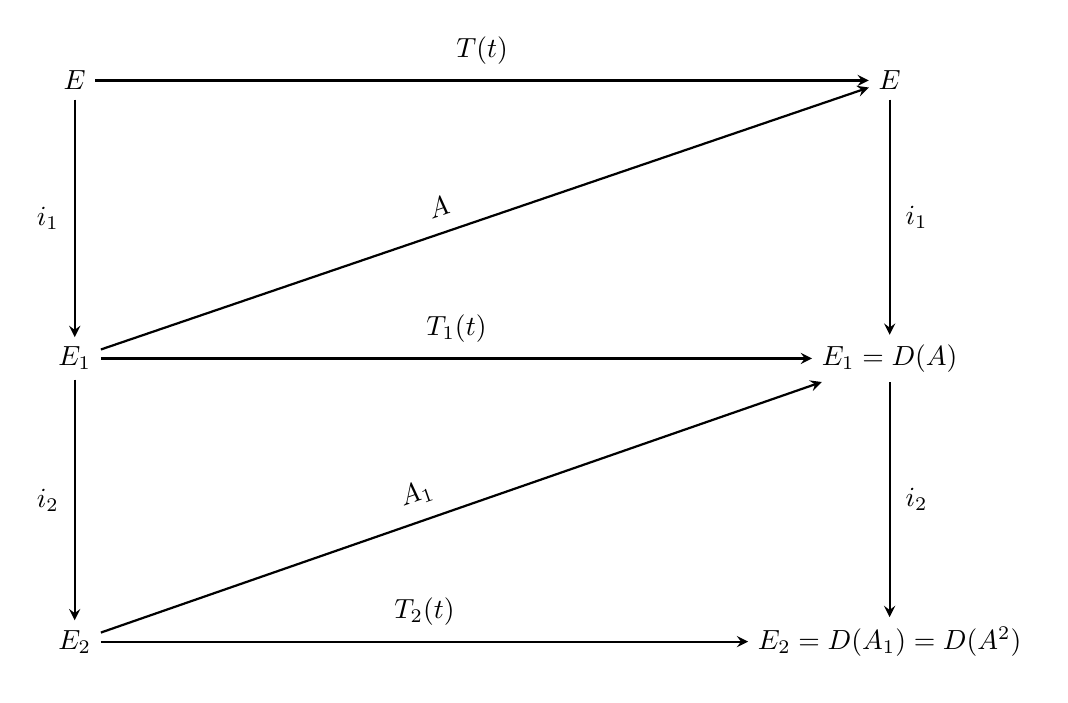
\begin{tikzpicture}[
    >=stealth,
    node distance=2.5cm,
    every node/.style={transform shape},
    label distance=3mm
]
    % Matrix mit verbessertem Spacing und Ausrichtung
    \matrix (m) [
        matrix of math nodes,
        row sep=3cm,    
        column sep=4cm, 
        nodes={anchor=center},
        nodes in empty cells
    ] {
        E & & E \\
        E_{1} & & E_{1} = D(A) \\
        E_{2} & & E_{2} = D(A_{1}) = D(A^{2}) \\
    };
    % Horizontale Pfeile mit einheitlicher Positionierung
    \draw[thick,->] (m-1-1) -- node[above=2pt] {$T(t)$} (m-1-3);
    \draw[thick,->] (m-2-1) -- node[above=2pt] {$T_{1}(t)$} (m-2-3);
    \draw[thick,->] (m-3-1) -- node[above=2pt] {$T_{2}(t)$} (m-3-3);
    % Vertikale Pfeile mit einheitlicher Beschriftung
    \draw[thick,->] (m-1-1) -- node[left=2pt] {$i_{1}$} (m-2-1);
    \draw[thick,->] (m-2-1) -- node[left=2pt] {$i_{2}$} (m-3-1);
    \draw[thick,->] (m-1-3) -- node[right=2pt] {$i_{1}$} (m-2-3);
    \draw[thick,->] (m-2-3) -- node[right=2pt] {$i_{2}$} (m-3-3);
    % Diagonale Pfeile mit verbesserter Platzierung
    \draw[thick,->] (m-2-1) -- node[above=2pt, sloped, pos=0.45] {$A$} (m-1-3);
    \draw[thick,->] (m-3-1) -- node[above=2pt, sloped, pos=0.45] {$A_{1}$} (m-2-3);
    % Gleichheitszeichen mit verbessertem Abstand
%    \node at ($(m-2-3)+(1.5,0)$) {$=$};
%    \node at ($(m-3-3)+(1.5,0)$) {$=$};
%    \node at ($(m-3-5)+(1.5,0)$) {$=$};
\end{tikzpicture}
\end{center}
%% --
%\newpage
%\begin{center}
%\begin{tikzpicture}[scale=1.5]
%% Nodes
%\node (E1) at (0,6) {$E$};
%\node (E2) at (4,6) {$E$};
%\node (E11) at (0,4) {$E_1$};
%\node (E12) at (4,4) {$E_1 = D(A)$};
%\node (E21) at (0,2) {$E_2$};
%\node (E22) at (4,2) {$E_2 = D(A_1) = D(A^2)$};
%\node (E31) at (0,0) {$E_3$};
%\node (E32) at (4,0) {$E_3$};
%
%% Horizontal arrows
%\draw[->] (E1) -- node[above] {$T(t)$} (E2);
%\draw[->] (E11) -- node[above] {$T_1(t)$} (E12);
%\draw[->] (E21) -- (E22);
%\draw[->] (E31) -- (E32);
%
%% Vertical arrows up
%\draw[->] (E11) -- node[left] {$i_1$} (E1);
%\draw[->] (E21) -- node[left] {$i_2$} (E11);
%\draw[->] (E31) -- node[left] {$i_3$} (E21);
%
%% Vertical arrows right side
%\draw[->] (E12) -- node[right] {$i_1$} (E2);
%\draw[->] (E22) -- node[right] {$i_2$} (E12);
%\draw[->] (E32) -- node[right] {$i_3$} (E22);
%
%% Diagonal arrows A
%\draw[->] (E1) -- node[above right] {$A$} (E12);
%\draw[->] (E11) -- node[above right] {$A_1$} (E22);
%\draw[->] (E21) -- node[above right] {} (E32);  % Unlabeled diagonal arrow
%\end{tikzpicture}
%\end{center}
%\newpage
%% --
For the translation semigroup on $L^{p}(\R)$ (see 2.3) the above construction leads to the usual \emph{Sobolev spaces}.
Therefore we might call $E_{n}$ the \emph{n-th Sobolev space} and $(T_{n}(t))_{t \geq 0}$ the \emph{n-th Sobolev semigroup} associated to $E$ and $(T(t))_{t \geq 0}$.
%% --
\begin{remark}\label{rem:a1-19.1}
\index{Sobolev spaces}
\index{Semigroups!Sobolev}
For $\lambda \in \rho(A)$ the operator $(\lambda - A)$ and the resolvent $R(\lambda,A)$ are isomorphisms from $E_{1}$ onto $E$, \resp from $E$ onto $E_{1}$ (show that $\|\cdot\|_{1}$ and $\|\cdot\|_{\lambda}$ with $\|\cdot\|_{\lambda} \coloneqq \|(\lambda - A)\cdot\|$ are equivalent).
%% --
In addition, the following diagram commutes. 
%% --
%\begin{tikzpicture}
%\matrix (m) [matrix of math nodes, row sep=3em, column sep=4em]
%{
%    E & & E \\
%    E_{1} & & E_{1} \\
%};
%\path[-stealth]
%(m-1-1) edge node[above] {$T(t)$} (m-1-3)
%(m-2-1) edge node[above] {$T_{1}(t)$} (m-2-3)
%(m-1-1) edge node[left] {$\lambda-A$} (m-2-1)
%(m-1-3) edge node[right] {$R(\lambda,A)$} (m-2-3);
%\end{tikzpicture}
%% --
\begin{center}
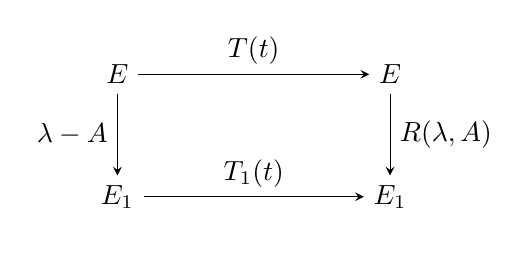
\begin{tikzpicture}[
    >=stealth,
    every node/.style={transform shape}
]
    % Matrix mit optimiertem Spacing
    \matrix (m) [
        matrix of math nodes,
        row sep=3em,    
        column sep=4em,
        nodes={anchor=center}
    ] {
        E    & & E \\
        E_{1}  & & E_{1} \\
    };
    % Pfeile als Pfad mit verbesserter Positionierung
    \path[->]
        (m-1-1) edge node[above] {$T(t)$} (m-1-3)
        (m-2-1) edge node[above] {$T_{1}(t)$} (m-2-3)
        (m-1-1) edge node[left] {$\lambda-A$} (m-2-1)
        (m-1-3) edge node[right] {$R(\lambda,A)$} (m-2-3);
    
\end{tikzpicture}
\end{center}
%% --
Therefore all Sobolev semigroups $(E_{n}, T_{n}(t))_{t \geq 0}$, $n \in \N$, are isomorphic.
\end{remark}
%% --
\begin{remark}\label{rem:a1-19.2}
For $\lambda \in \rho(A)$ consider the norm
%% --
\[
    \|f\|_{-1} \coloneqq \|R(\lambda,A)f\|
\]
%% --
for every $f \in E$ and define $E_{-1}$ as the completion of $E$ for $\|\cdot\|_{-1}$.
\end{remark}
%% --
Then $(T(t))_{t \geq 0}$ extends continuously to a strongly continuous semigroup $(T_{-1}(t))_{t \geq 0}$ on $E_{-1}$ and the above diagram can be extended to the negative integers.
%% --
\section{The $\mathcal{F}$-Product Semigroup}\label{sec:a1-3.6}
\index{$\mathcal{F}$-Product}
\index{$\mathcal{F}$-Product!Semigroup}
%% --
It is standard in functional analysis to consider a sequence of points in a certain space as a point in a new and larger space.
In particular such a method can serve to convert an approximate eigenvector of a linear operator into an eigenvector.
Occasionally we will need such a construction and refer to Section V.1 of \citet{schaefer:1974}. 

If we try to adapt this construction to strongly continuous semigroups we encounter the difficulty that the semigroup extended to the larger space will not remain strongly continuous.
An idea already used in 3.4 will help to overcome this difficulty.

Let $\mathcal{T} = (T(t))_{t \geq 0}$ be a strongly continuous semigroup on the Banach space $E$.
Denote by $m(E)$ the Banach space of all bounded $E$-valued sequences endowed with the norm
%% --
\[
    \|(f_{n})_{n \in \N}\| \coloneqq \sup \{\|f_{n}\| \colon n \in \N\} .
\]
%% --
It is clear that every $T(t)$ extends canonically to a bounded linear operator
%% --
\[
    \hat{T}(t)(f_{n}) \coloneqq (T(t)f_{n})
\]
%% --
on $m(E)$, but the semigroup $(\hat{T}(t))_{t \geq 0}$ is strongly continuous if and only if $T$ has a bounded generator.
Therefore we restrict our attention to the closed, $(\hat{T}(t))$-invariant subspace
%% --
\[
    m^{\mathcal{T}}(E) \coloneqq \{(f_{n}) \in m(E) \colon \lim_{t \to 0} \|T(t)f_{n}-f_{n}\| = 0 \text{ uniformly for } n \in \N\} .
\]
%% --
Then the restricted semigroup
%% --
\[
    \hat{T}(t)(f_{n}) = (T(t)f_{n}), \quad (f_{n}) \in m^{\mathcal{T}}(E)
\]
%% --
is strongly continuous and we denote its generator by $(\hat{A},D(\hat{A}))$.

The following lemma shows that $\hat{A}$ is obtained canonically from $A$.
%% --
\begin{lemma}\label{lem:a1-3.6}
For the generator $\hat{A}$ of $(\hat{T}(t))_{t \geq 0}$ on $m^{\mathcal{T}}(E)$ one has the following properties.
%% --
\begin{enumerate}[(i)]

\item 
$D(\hat{A}) = \{(f_{n}) \in m^{\mathcal{T}}(E) \colon f_{n} \in D(A) \text{ and } (Af_{n}) \in m^{\mathcal{T}}(E)\}$,

\item 
$\hat{A}(f_{n}) = (Af_{n})$ for $(f_{n}) \in D(\hat{A})$ .
\end{enumerate}

\end{lemma}
%% --
For the proof we refer to Lemma 1.4. of \citet{derndinger:1980}.

Now let $\mathcal{F}$ be any filter on $\N$ finer than the Frechét filter (i.e.\xspace the filter of sets with finite complement. In most cases $F$ will be either the Frechét filter or some free ultra filter.)
%% --
The space of all $\mathcal{F}$-null sequences in $m(E)$, i.e.\xspace
%% --
\[
    c_{\mathcal{F}}(E) \coloneqq \{(f_{n}) \in m(E) \colon \mathcal{F}\text{-}\lim\|f_{n}\| = 0\}
\]
%% --
is closed in $m(E)$ and invariant under $(\hat{T}(t))_{t \geq 0}$. 
We call the quotient spaces
%% --
\[
    E_{\mathcal{F}} \coloneqq m(E)/c_{\mathcal{F}}(E) \quad \text{and} \quad E_{\mathcal{F}}^{T} \coloneqq m^{\mathcal{T}}(E)/c_{\mathcal{F}}(E)\cap m^{\mathcal{T}}(E)
\]
%% --
the \emph{$\mathcal{F}$-product of $E$} and the \emph{$ \mathcal{F} $-product of $E$ with respect to the semigroup $T$}, respectively.

Thus $E_{\mathcal{F}}^{T}$ can be considered as a closed linear subspace of $E_{\mathcal{F}}$. 
We have $E_{\mathcal{F}}^{T} = E_{\mathcal{F}}$ if (and only if) $T$ has a bounded generator.

The canonical quotient norm on $E_{\mathcal{F}}$ is given by
%% --
\[
    \|(f_{n}) + c_{\mathcal{F}}(E)\| = \mathcal{F}\text{-}\lim \sup \|f_{n}\| .
\]
%% --
We can apply Subsec.\;\ref{subsec:a1-3.3} in order to define the \emph{$\mathcal{F}$-product semigroup} $(T_{\mathcal{F}}(t))_{t \geq 0}$ on $E_{\mathcal{F}}^{T}$ by
%% --
\[
    T_{\mathcal{F}}(t)((f_{n}) + c_{\mathcal{F}}(E)) \coloneqq (T(t)f_{n}) 
    	+ c_{\mathcal{F}}(E)\cap m^{\mathcal{T}}(E)
\]
%% --
Thus $T_{\mathcal{F}}(t)$ is the restriction of $T(t)_{F}$ where $T(t)_{F}$ denotes the canonical extension of $T(t)$ to the $\mathcal{F}$-product $E_{\mathcal{F}}$. 
But note that $(T(t)_{F})_{t \geq 0}$ is not strongly continuous unless $T$ has a bounded generator.

With the canonical injection $j \colon f \mapsto (f,f,f,\ldots) + c_{\mathcal{F}}(E)$ from $E$ into $E_{\mathcal{F}}^{T}$ the operators $T_{\mathcal{F}}(t)$ are extensions of $T(t)$ satisfying $\|T_{\mathcal{F}}(t)\| = \|T(t)\|$. The basic facts about the generator $(A_{\mathcal{F}},D(A_{\mathcal{F}}))$ of $(T_{\mathcal{F}}(t))_{t \geq 0}$ follow from 3.3 and are collected in the following proposition.
%% --
\begin{proposition}\label{prop:a1-3.6}
For the generator $(A_{\mathcal{F}},D(A_{\mathcal{F}}))$ of the $\mathcal{F}$-product semigroup the following holds.
%% --
\begin{enumerate}[(i)]
\item 
$D(A_{\mathcal{F}}) = \{(f_{n}) + c_{\mathcal{F}}(E) \colon f_{n} \in D(A); (f_{n}), (Af_{n}) \in m^{\mathcal{T}}(E)\}$,

\item 
$A_{\mathcal{F}}((f_{n}) + c_{\mathcal{F}}(E)) = (Af_{n}) + c_{\mathcal{F}}(E)$.

\end{enumerate}
\end{proposition}
%% --
In case $A$ is a bounded operator then $D(A_{\mathcal{F}}) = E_{\mathcal{F}}^{T} = E_{\mathcal{F}}$ and $A_{\mathcal{F}}$ is the canonical extension of $A$ to $E_{\mathcal{F}}$.

We will show in A-III,4.5 that the above construction preserves and even improves many spectral properties of the semigroup and its generator.

%% --
\section{The Tensor Product Semigroup}\label{sec:a1-3.7}
\index{Tensor Product}
\index{Tensor Product!Semigroup}
%% --
Real- or complex-valued functions of two variables $x$, $y$ are often limits of functions of the form $\sum_{i=1}^{n} f_{i}(x)g_{i}(y)$ which, to some extent, allows one to consider the variables $x$ and $y$ separately.
Since algebraic manipulation with these latter functions is governed by the formal rules of a tensor product, it is customary to identify (for example) the function
%% --
\[
    (x,y) \mapsto f(x)g(y)
\]
%% --
with the tensor product $f \otimes g$ and to consider limits of linear combinations of such functions as elements of a completed tensor product.

To be more precise, we briefly present the most important examples for this situation.
%% --
\begin{examples}\label{ex:a1-5.1}
\index{Tensor Product!Examples}
%% --
\begin{enumerate}[(i), wide, labelsep=1em, itemindent=\parindent]

\item
Let $(X,\Sigma,\mu)$ and $(Y,\Omega,\nu)$ be measure spaces. 
If we identify for $f_{i} \in L^{p}(\mu)$, $g_{i} \in L^{p}(\nu)$ the elements $\sum_{i=1}^{n} f_{i} \otimes g_{i}$ of the tensor product
%% --
\[
    L^{p}(\mu) \otimes L^{p}(\nu)
\]
%% --
with the (class of $\mu \times \nu$-a.e.-defined) functions
%% --
\[
    (x,y) \mapsto \sum_{i=1}^{n} f_{i}(x)g_{i}(y) ,
\]
%% --
then $L^{p}(\mu) \otimes L^{p}(\nu)$ becomes a dense subspace of $L^{p}(X\times Y,\Sigma\times\Omega,\mu\times\nu)$ for $1 \leq p < \infty$.

\item
Similarly, let $X$,$Y$ be compact spaces. Then $C(X) \otimes C(Y)$ becomes a dense subspace of $C(X\times Y)$ by identifying, for $f \in C(X)$ and $g \in C(Y)$, $f \otimes g$ with the function
%% --
\[
    (x,y) \mapsto f(x)g(y) .
\]
%% --
\end{enumerate}
\end{examples}
%% --
We do not intend to go deeper into the quite sophisticated problems related to normed tensor products of general Banach spaces, but will rather confine ourselves to the discussion of certain special cases.
These will always be related to one of the following standard methods to define a norm on the tensor product of two Banach spaces $E$, $F$.

Let $u \coloneqq \sum_{i=1}^{n} f_{i} \otimes g_{i}$ be an element of $E \otimes F$. 
Then
%% --
\begin{enumerate}[(i), wide, labelsep=1em, itemindent=\parindent]

\item
$\|u\|_{\pi} \coloneqq \inf\{\sum_{j=1}^{m} \|h_{j}\|\|k_{j}\| \colon u = \sum_{j=1}^{m}h_{j} \otimes k_{j}, h_{j} \in E, k_{j} \in F\}$ defines the \emph{greatest cross norm $\pi$} on $E \otimes F$.

\item
$\|u\|_{\epsilon} \coloneqq \sup\{\langle u,\phi \otimes \psi\rangle \colon \phi \in E', \psi \in F', \|\phi\|, \|\psi\| \leq 1\}$ defines the 
\emph{least cross norm $\epsilon$} on $E \times F$. 
Here, $\langle u,\phi \otimes \psi\rangle$ denotes the canonical bilinear form on $(E \otimes F) \times (E' \otimes F')$, i.e.\xspace, $\langle\sum_{i=1}^{n} f_{i} \otimes g_{i},\phi \otimes \psi\rangle = \sum_{i=1}^{n} \langle f_{i},\phi\rangle\langle g_{i},\psi\rangle$.

\item
if $E$ and $F$ are Hilbert spaces, $\|u\|_{h} = (u|u)_{h}^{1/2}$, where the scalar product $(\cdot|\cdot)_{h}$ is defined as in (ii), defines the \emph{Hilbert norm $h$} on $E \otimes F$.
\end{enumerate}
%% --
In the following we write $E \otimes_{\alpha} F$ for the tensor product of $E$ and $F$ endowed---if applicable---with one of the norms $\pi$, $\epsilon$, $h$ just defined.
In each case one has $\|f \otimes g\| = \|f\|\|g\|$ for $f \in E$, $g \in F$.

By $E \widetilde{\otimes}_{\alpha} F$ we mean the completion of $E \otimes_{\alpha} F$. 
Moreover we recall how examples (i) and (ii) above fit into this pattern
%% --
\[
    L^{1}(\mu \otimes \nu) = L^{1}(\mu) \widetilde{\otimes}_{\pi} L^{1}(\nu), 
    \quad L^{2}(\mu \otimes \nu) = L^{2}(\mu) \widetilde{\otimes}_{h} L^{2}(\nu),
\]
\[
    C(X \otimes Y) = C(X) \widetilde{\otimes}_{\epsilon} C(Y).
\]
%% --
Finally, we point out that for any $S \in \LE$, $T \in \L{F} $, the mapping
%% --
\[
    \sum_{i=1}^{n}f_{i} \otimes g_{i} \mapsto \sum_{i=1}^{n}Sf_{i} \otimes Tg_{i}
\]
%% --
defined on $E \otimes F$ is linear and continuous on $E \otimes_{\alpha} F$, hence has a continuous extension to $ E \widetilde{\otimes}_{\alpha} F$. 
This operator, as well as its continuous extension, will be denoted by $S \otimes T$ and satisfies $\|S \otimes T\| = \|S\|\|T\|$. 
The notation $A \otimes B$ will also be used in the obvious way if $A$ and $B$ are not necessarily bounded operators on $E$ and $F$. 
We are now ready to consider semigroups induced on the tensor product.
%% --
\begin{proposition}\label{prop:a1-3.7}
Let $(S(t))_{t\geq 0}$ and $(T(t))_{t\geq 0}$ be strongly continuous semigroups on Banach spaces $E$, $F$, and let $A$, $B$ be their generators. 
Then the family $(S(t) \otimes T(t))_{t\geq 0}$ is a strongly continuous semigroup on 
$ E \widetilde{\otimes}_{\alpha} F $.
The closure of $A \otimes \Id + \Id \otimes B$, defined on the core $D(A) \otimes D(B)$, is its generator.
\end{proposition}
%% --
\begin{proof}
It is immediately verified that $(S(t)\otimes T(t))_{t\geq 0}$ is in fact a semigroup of operators on 
$ E \widetilde{\otimes}_{\alpha} F $. 
The strong continuity need only be verified at $t = 0$ and on elements of the form $u = f \otimes g \in E \otimes F$.

This verification being straightforward, there remains to show that the generator of $(S(t)\otimes T(t))_{t\geq 0}$ is obtained as the closure of 
%
\[
	(A \otimes \Id + \Id \otimes B,D(A) \otimes D(B)) .
\]
%
To this end, let $f \in D(A)$ and $g \in D(B)$. 
Then
%% --
\begin{align*}
    &\lim_{h\to 0} \frac{1}{h}(T(h) \otimes S(h)(f \otimes g)-f \otimes g) \\
    &= \lim_{h\to 0} \frac{1}{h}(T(h)f \otimes (S(h)g-g) + (T(h)f-f) \otimes g) \\
    &= (f \otimes Bg) + (Af \otimes g) .
\end{align*}
%% --
Since the elements of the form $f \otimes g$, $f \in D(A)$, $g \in D(B)$, generate the linear subspace $D(A) \otimes D(B)$ of $E \otimes_{\alpha} F$, this subspace belongs
%% --
%\newpage
%% -- a1-25
to the domain of the generator.
Moreover, $D(A) \otimes D(B)$ is dense in $E \widetilde{\otimes}_{\alpha} F$ and invariant under $(S(t)\otimes T(t))_{t\geq 0}$, hence it is a core of $A \otimes \Id + \Id \otimes B$ by Prop.~\ref{prop:a1-1.9}\,(ii).
\end{proof}
%% --
\section{The Product of Commuting Semigroups}\label{sec:a1-3.8}
%\index{Product of Semigroups}
\index{Tensor Product!Commuting Semigroups}

Let $(S(t))_{t\geq 0}$ and $(T(t))_{t\geq 0}$ be semigroups with generators $A$ and $B$, respectively on some Banach space $E$.
It is not difficult to see that the following assertions are equivalent.
%% --
\begin{enumerate}[(a), leftmargin=2em]

\item 
$S(t)T(t) = S(t)T(t)$ for all $t \geq 0$.

\item 
$R(\mu,A)R(\mu,B) = R(\mu,B)R(\mu,A)$ for some $\mu \in \rho(A) \cap \rho(B)$.

\item 
$R(\mu,A)R(\mu,B) = R(\mu,B)R(\mu,A)$ for all $\mu \in \rho(A) \cap \rho(B)$.

\end{enumerate}
%% --
In that case $U(t) = S(t)T(t)$ $(t \geq 0)$ defines a semigroup $(U(t))_{t\geq 0}$.
Using %Prop.~\ref{prop:a1-1.9}\,(ii).
Prop.~\ref{prop:a1-1.9}\,(ii) on p.~\pageref{prop:a1-1.9} 
one easily shows that $D_{0} \coloneqq D(A) \cap D(B)$ is a core for its generator $C$ and $Cf = Af + Bf$ for all $f \in D_{0}$.

\section*{Notes}
\addcontentsline{toc}{section}{Notes}
\index{Notes!Semigroup Theory}

For more complete information on semigroup theory we refer the reader to \citet{hillephillips:1957}, to the monographs by \citet{davies:1980}, 
\citet{goldstein:1985a} and \citet{pazy:1983}, to the survey article by \citet{kreinkhazan:1985}, to the bibliography by 
\citet{goldstein:1985b} and to \citet{engelnagel:2006}.

%% --
%\bibliographystyle{abbrvnat}
%\bibliography{bib/ln-references}
%
%\bibliographystyle{spmpsci}
\begin{thebibliography}{11}
\providecommand{\natexlab}[1]{#1}
\providecommand{\url}[1]{\texttt{#1}}
\expandafter\ifx\csname urlstyle\endcsname\relax
  \providecommand{\doi}[1]{doi: #1}\else
  \providecommand{\doi}{doi: \begingroup \urlstyle{rm}\Url}\fi

\bibitem[Davies(1980)]{davies:1980}
E.~Davies.
\newblock \emph{One-parameter Semigroups}.
\newblock Academic Press, London-New York-San Francisco, 1980.

\bibitem[Engel and Nagel(2000)]{engelnagel:2000}
K.-J. Engel and R.~Nagel.
\newblock \emph{One-Paramter Semigroups for Linear Evolution Equations}.
\newblock Number 194 in Graduate Textes in Mathematics. Springer, Berlin AND
  Heidelberg AND New York, 2000.

\bibitem[Goldstein(1985{\natexlab{a}})]{goldstein:1985a}
J.~Goldstein.
\newblock \emph{Semigroups of Operators and Applications}.
\newblock Oxford University Press, 1985{\natexlab{a}}.

\bibitem[Goldstein(1985{\natexlab{b}})]{goldstein:1985b}
J.~Goldstein.
\newblock A (more-or-less) complete bibliography of semigroups of operators
  through 1984.
\newblock Preprints and lecture notes in mathematics, Tulane University,
  1985{\natexlab{b}}.

\bibitem[Hille and Phillips(1957)]{hillephillips:1957}
E.~Hille and R.~S. Phillips.
\newblock \emph{Functional Analysis and Semigroups}, volume~31 of
  \emph{Colloquium Publications}.
\newblock American Mathematical Society, Providence, R.I., 1957.

\bibitem[Kato(1966)]{kato:1966}
T.~Kato.
\newblock \emph{Perturbation Theory for Linear Operators}.
\newblock Springer, 1966.
\newblock 2nd printing: Berlin-Heidelberg-New York: Springer 1976.

\bibitem[Krein and Khazan(1985)]{kreinkhazan:1985}
S.~G. Krein and M.~I. Khazan.
\newblock Differential equations in a banach space.
\newblock \emph{J. Soviet Math.}, 30\penalty0 (3):\penalty0 2154--2239, 1985.
\newblock \doi{10.1007/BF02105398}.
\newblock URL \url{https://doi.org/10.1007/BF02105398}.

\bibitem[Pazy(1983)]{pazy:1983}
A.~Pazy.
\newblock \emph{Semigroups of Linear Operators and Applications to Partial
  Differential Equations}.
\newblock Springer, Berlin-Heidelberg-New York-Tokyo, 1983.

\bibitem[Phillips(1954)]{phillips:1954}
R.~S. Phillips.
\newblock A note on the abstract {Cauchy} problem.
\newblock \emph{Proc. Nat. Acad. Sci. U.S.A.}, 40:\penalty0 244--248, 1954.

\bibitem[Reed and Simon(1975)]{reedsimon:1975}
M.~Reed and B.~Simon.
\newblock \emph{Methods of Modern Mathematical Physics {II}. {Fourier}
  Analysis, Self-Adjointness}.
\newblock Academic Press, New York, 1975.

\bibitem[Schaefer(1974)]{schaefer:1974}
H.~H. Schaefer.
\newblock \emph{Banach Lattices and Positive Operators}.
\newblock Springer, New York-Heidelberg-Berlin, 1974.

\end{thebibliography}




%% -- Literatur
%% --

% -- ln-references.bib im gleichen Verzeichnis
%% -- oder im TeX-Baum texmf/bibtex/bib
%% --
%\RaggedRight
\bibliography{ln-references} 

%% -- Index
%% --

\clearpage
\printindex

%% --
\end{document}









